\documentclass[../main.tex]{subfiles}

\begin{document}
We implemented the tsunami simulation for the 1D case.  We use the surface \ref{1DLine} to simulate the tsunami given an initial perturbation. 

\begin{figure}[H]
\centering
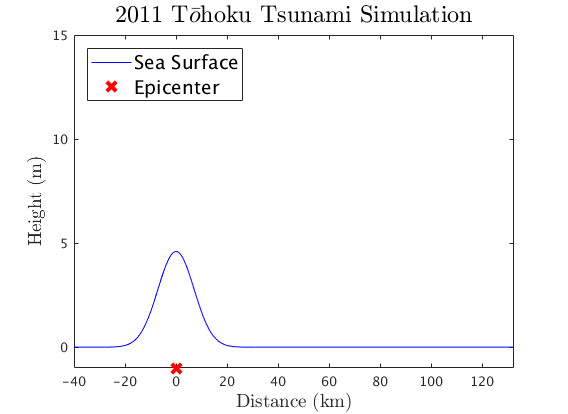
\includegraphics[scale = 0.5]{tsunami_init.png}
\end{figure}

When the simulation begins, we see the perturbation split into two separate waves, one that travels to the power plant and one that travels away.  We notice that as we had expected, the wave that is travelling towards the power plant becomes taller and slows down in speed.  The wave moving away will flatten out and increase its speed.  

\begin{figure}[H]
\centering
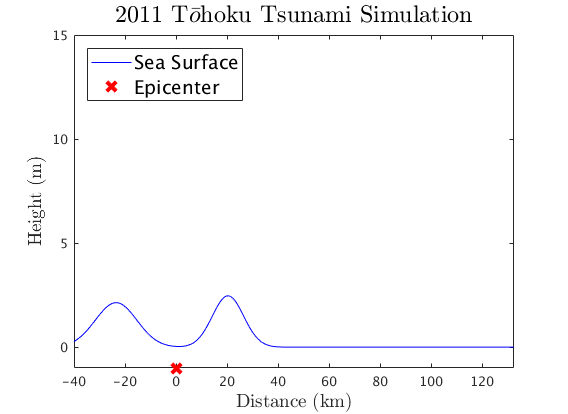
\includegraphics[scale = 0.5]{tsunami_split.png}
\end{figure}


As the tsunami approaches the power plant, we examine the change in the wave's height.  Reports indicate that the tsunami reached a height of 15 meters by the time it reached the power plant site \cite{nuclearAssociation}.  In our simulation, the tsunami's height changes significantly when it arrives to near-shore.  Due to the seafloor approaching sea level, we see the tsunami rapidly grow in height and decrease speed.  In fact, at the end of the simulation when the right edge of the tsunami
reaches the coast, we see that in fact the height of the tsunami reaches 15 meters.

\begin{figure}[H]
\centering
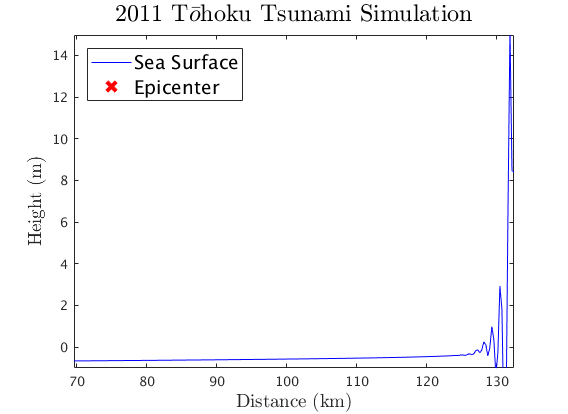
\includegraphics[scale = 0.5]{tsunami_final.png}
\end{figure}

The result of our simulation validates our assumptions and data derived in 2011 at the power plant.  We see that the tsunami in fact reaches the expected height at coast, and we were effectively able to model the tsunami wave.


\end{document}
